% File acl2020.tex
%
%% Based on the style files for ACL 2020, which were
%% Based on the style files for ACL 2018, NAACL 2018/19, which were
%% Based on the style files for ACL-2015, with some improvements
%%  taken from the NAACL-2016 style
%% Based on the style files for ACL-2014, which were, in turn,
%% based on ACL-2013, ACL-2012, ACL-2011, ACL-2010, ACL-IJCNLP-2009,
%% EACL-2009, IJCNLP-2008...
%% Based on the style files for EACL 2006 by 
%%e.agirre@ehu.es or Sergi.Balari@uab.es
%% and that of ACL 08 by Joakim Nivre and Noah Smith

\documentclass[11pt,a4paper]{article}
\usepackage[hyperref]{acl2020}
\usepackage{times}
\usepackage{latexsym}
\usepackage{amsfonts}
\usepackage{amsmath}
\usepackage{graphicx}

\renewcommand{\UrlFont}{\ttfamily\small}

% This is not strictly necessary, and may be commented out,
% but it will improve the layout of the manuscript,
% and will typically save some space.
\usepackage{microtype}

\aclfinalcopy % Uncomment this line for the final submission
%\def\aclpaperid{***} %  Enter the acl Paper ID here

%\setlength\titlebox{5cm}
% You can expand the titlebox if you need extra space
% to show all the authors. Please do not make the titlebox
% smaller than 5cm (the original size); we will check this
% in the camera-ready version and ask you to change it back.

\newcommand\BibTeX{B\textsc{ib}\TeX}

\title{Multi-Agent Reinforcement Learning in Zombie-Survival Games}

\author{Peter Hollows \\
  \texttt{stanford@dojo7.com} \\\And
  Mark Presser \\
  \texttt{mark.presser95@gmail.com} \\}

\date{}

\begin{document}
\maketitle
\begin{abstract}
  The abstract goes here...
\end{abstract}

\section{Introduction}

Reinforcement Learning (RL) methods are seeing increasing use in real-world control systems.
In part, the rising popularity of RL methods is due to its widely publicized success on challenging tasks,
as well as the availability of quality open-source frameworks containing implementations of state-of-the-art models.

\subsection{Closing the Reality Gap}

Current RL methods are not sample-effecicient, meaning the policy learner needs a lot of data before an effective policy can be found.
Often, there is not enough data available, or it cannot be captured safely (consider an autonomous driver learning the best policy for a near-crash scenario, where it will make mistakes in order to learn).
To work around these issues, RL policies intended for real-world control tasks are usually trained in simulated environments before being further trained or deployed in the real-world.

However, simulations often do not capture all the relevant real-world dynamics, so it can be difficult to transition a policy from the simulator to reality.
This difficulty, known as the "reality gap", is often mitigated by adding noise to the simulation (to mimic noisy sensors and stochastic dynamics),
or by sufficiently improving the simulation to model the relevant dynamics.

This approach has enjoyed success in single-agent RL settings like autonomous aircraft and robotics.

\subsection{Multi-Agent RL}

In cooperative settings like factories, or competitive settings like markets, using the simulation technique becomes more challenging;
simulating the dynamics of other agents present in the environment is a difficult problem, even in simulation.
This is especially the case when the policies of multiple agents are being modified and improved at the same time.

These issues in multi-agent settings motivated a training algorithm called Multi-Agent Deep Deterministic Policy Gradient (MADDPG).
MADDPG addresses some issues in multi-agent learning, and allows running experiments that explore the emergence of policies competitive and cooperative policies in complex environments.

\subsection{Environmental Dynamics}

We explore MADDPG in the context of a mixed competitive-cooperative simulated environment called Zombie-Survival game under multiple scenarios.
In these scenarios we show how specific kinds of environmental dynamics can affect large (and sometimes surprising and unintended) changes in the evolution of policies.
We present methods and results for each scenario, and conclude with a discussion (\ref{sec:discussion}) on safety issues we feel apply to a wide array of RL systems.

\subsection{Overview}

In (\ref{sec:background}) we review theory, RL algorithms, and aspects of agent design.
In (\ref{sec:game}) we detail the basic simulation environment.
In (\ref{sec:baseline}) we detail the experimental setup and initial results.
In (\ref{sec:anon}) we investigate partial observability, and how compression of the observation function can speed policy discovery.
In (\ref{sec:health}) we alter the environment to cause a change in the value function (keeping reward unchanged) to study the impact on learned policies.
In (\ref{sec:arms}) we arm the survivors with projectile weapons to investigate how additional capability can make it harder for agents to achieve their objectives.

\section{Background}
\label{sec:background}

\subsection{The Markov Decision Process}

A Markov Decision Process (MDP) formalizes the interaction of an agent with an environment.
At every time step, an \emph{agent} receives observations of the \emph{state} of the \emph{environment}, and sends \emph{actions} to the environment.
The environment transitions from one state to the next over time, and actions from the agent can influence which states the environment transitions to.
At every time step, the agent receives a \emph{reward} based on the state of the environment.
In the case when state transitions are not independent (i.e. the chance of arriving in a state depends on visiting previous states), then agent actions in a state can impact future expected rewards as well as immediate rewards.

RL algorithms attempt to solve the MDP in order to maximize return (reward over time).
This can be done by learning a policy (a function that maps from state to action).
A policy can often be learned directly, or by learning a value function (a mapping from states and actions to expected returns) from which a policy can be extracted.

\subsection{DDPG}

Q-Learning is a popular RL method that makes use of an action-value function $Q^\pi(s, a)$ corresponding to a policy $\pi$ (where $s$ is the state, and $a$ the action).
Deep Q-Learning learns (DQN) learns the action-value function $Q^*$ corresponding to the optimal policy by minimizing the loss function
\begin{equation}
  \mathcal{L}(\theta)=\mathbb{E}_{s,a,r,s'}[(Q^*(s,a|\theta)-y)^2],
\end{equation}
where $y=r+\gamma\max_{a'}\bar{Q}^*(s',a')$,
by repeatedly adjusting the parameters $\theta$ of the target action-value function $\bar{Q}$.
The Q-function can be expressed as $Q^{\pi}(s,a)=\mathbb{E}[R|s,a]$, where $R_t$ is the discounted sum of future rewards at time $t$, given by: $R_t=\sum_{k=t}^\infty\gamma(k-t)r_k$.
To reduce the variance of estimates for the above expectation, Q-Learning often makes use of an Experience Replay (ER) buffer that stores the experiences of many state transitions.

Policy-gradient (PG) methods learn a policy $\pi_\theta$, parameterized by $\theta$,
by sampling the gradient of a performance measure $J(\theta)$ with respect to $\theta$.

\begin{equation}
  \nabla_\theta J(\theta)=\mathbb{E}_\pi\left[Q^\pi(s, a) \frac{\nabla_\theta\pi_\theta(a|s)}{\pi_\theta(a|s)}\right]
\end{equation}

REINFORCE, a simple PG algorithm, uses all the steps in an episode to find $Q^\pi(s,a)=\mathbb{E}_\pi[G|s,a]$, where $G$ is the total reward of an episode.
Because reward functions sometimes give high values for some states, this method can give high variance gradient estimates.
This can be remedied by using a baseline $b(s)$:

\begin{equation}
  \nabla_\theta J(\theta)=\mathbb{E}_\pi\left[(G-b(s)) \frac{\nabla_\theta\pi_\theta(a|s)}{\pi_\theta(a|s)}\right]
\end{equation}

Actor-Critic (AC) improves on REINFORCE by learning a state-value function with baseline (critic), and an action-value function (actor) concurrently.
AC also has the advantage that the parameters for both functions are updated at every step in an episode.
The policy gradient at each time step $t$ can be expressed:

\begin{equation}
  \nabla_\theta J(\theta)=\mathbb{E}_\pi\left[\delta_t \frac{\nabla_\theta\pi_\theta(a|s)}{\pi_\theta(a|s)}\right]
\end{equation}
\begin{equation}
  \delta_t = r_{t+1}+\gamma \hat{v}(s_{t+1}, w)-\hat{v}(s_t,w)
\end{equation}

where $\gamma$ is a discount parameter, and $\hat{v}(w)$ the state-value function with parameters $w$.

Deterministic Policy Gradient (DPG) methods extend policy gradient to deterministic policies.
A deterministic policy ($\mu_\theta$) maps a state to an action,
whereas a stochastic policy ($\pi_\theta$) provides a conditional probability of an action in a given state.

\begin{equation}
  \nabla_\theta J(\theta)=\mathbb{E}_s\left[\nabla_\theta \mu_\theta(a|s) \nabla_a Q^\mu(s,a)|_{a=\mu_\theta(s)}\right]
\end{equation}

DPG methods are often used in continuous control tasks
(taking the gradient of $Q^\mu$ with respect to $a$ requires the action space to be continuous).

Deep Deterministic Policy Gradient (DDPG) combines ideas from DPG and DQN.
In DDPG the actor and critic are approximated with neural networks.
DDPG uses target networks for both actor and critic, and makes use of an experience replay buffer to store agent trajectories.

\subsection{MADDPG}

The Markov Decision Process (MDP) framework regards other agents as part of the environment from the perspective of a single agent.
From the perspective of an agent, the influence on rewards from other agents in the environment can make it harder to learn a policy;
this is especially so when the environment contains other agents that are also learning policies,
because elements of the `environment' change while the agent is trying to learn them.

It was shown in () that the chance of sampling a policy-gradient update in an improved direction decreases exponentially with the number of agents being trained in the shared environemnt.

MADDPG addresses this stabilitiy issue by using centralized critics.
In MADDPG, the critic $Q^\pi_i(x, a_1, a_2, ..., a_N)$ for agent $i$ has access to the actions of all $N$ agents, and some state information $x$.
The critic is often only used in training, so it's possible to deploy MADDPG actors in continuous control tasks where knowledge of other actors' actions are not available.
Agents can have different state and action spaces, and be goverened by different reward functions.
We use the MADDPG algorithm for all agents within our scenarios.

\subsection{Agent design}

When implementing an RL system there are many important design considerations:

\begin{itemize}
  \item \emph{Algorithm}: Different algorithms are suited to different tasks. A selected algorithm will need to perform well with the selected action-space, state-space, reward function and environmental dynamics.
  \item \emph{State-space}: The state-space describes how environmental observations are presented to the algorithm. Constructing the correct, relevant abstractions allow an agent to better learn the environment.
  \item \emph{Action-space}: The action-space describes actions available to the agent. The level of abstraction here should be fine enough for precise control, but general enough for a policy to be learnable.
  \item \emph{Reward function}: The reward function provides a scalar feedback value (positive or negative) to the agent. Most algorithms assume the reward signal contains no noise, and require point-estimates rather than a distribution. Crafting a consistent reward function that reflects the exact desires of the designer can be challenging. Some algorithms can infer the a reward function from feedback, but most will try to maximize explicit reward.
\end{itemize}

We examine the imapct of design choices for state-space, action-space, and reward function in our scenarios.

\section{Scenarios}
\label{sec:scenarios}

\subsection{Zombie-Survival Game}
\label{sec:game}

The Zombie-Survival scenarios cover a set of games simulating survivors and zombies in a zombie-apocalypse scenario.
When a zombie is in physical contact with a survivor this results in a `bite' between zombie and survivor.
Zombies attempt to bite survivors and are rewarded for each step they are in contact.
Survivors attempt to distance themselves from zombies and are penalized every time they are bitten.
Survivors can suffer a bite from multiple zombies in the same time step.

Zombies have the advantage of numbers (there are 5 zombies and 2 survivors), whereas survivors have the advantage of faster accleration and a higher maximum speed.
All reward functions are independent, agents do not share reward.
The game offers a scenario with asymmetric power dynamics between competitive teams, and allows the emergence of compeitive or cooperative behavior within a team.

\begin{table}
\centering
\begin{tabular}{lrr}
\hline \textbf{Setting} & \textbf{Survivors} & \textbf{Zombies} \\ \hline
  world size ($m$) & 2x2 & 2x2 \\
  timestep ($s$) & 0.1 & 0.1 \\
  episode length ($s$) & 10 & 10 \\
  num. agents & 2 & \textbf{5} \\
  agent radius ($m$) & 0.05 & 0.05 \\
  agent mass ($kg$) & 1.0 & 1.0 \\
  acceleration ($ms^-2$) & \textbf{4.0} & 3.0 \\
  max. speed ($ms^-1$) & \textbf{1.3} & 1.0 \\
  bite reward & -10 & +10 \\
\hline
\end{tabular}
\caption{\label{game-settings} Scenario settings. }
\end{table}

\subsection{Scenario: Baseline}
\label{sec:baseline}

We modify the 'Predator-prey' particle environment from (), which implements a multi-agent environment with a continuous action-space, a fully-observable state-space, and basic 2D physics.
Each agent is represented as a circle that has mass, position, velocity, velocity dampening, maximum acceleration, and maximum speed.
%Actions are 4D discrete (softmax probabilities) which are mapped to 2D continuous force vectors to control movement.
The predator-prey environment uses reward shaping to discourage agents from moving out of bounds.
We remove this additional term in the reward function and implement fixed boundary walls.
We implement the biting rules, modify the agent count and adjust the agents' physical capabilities (see Table \ref{game-settings}).
We run several training jobs for 10,000 steps each to capture the emergence of different policies.

\subsection{Results: Baseline}

\begin{figure}
  \centering
  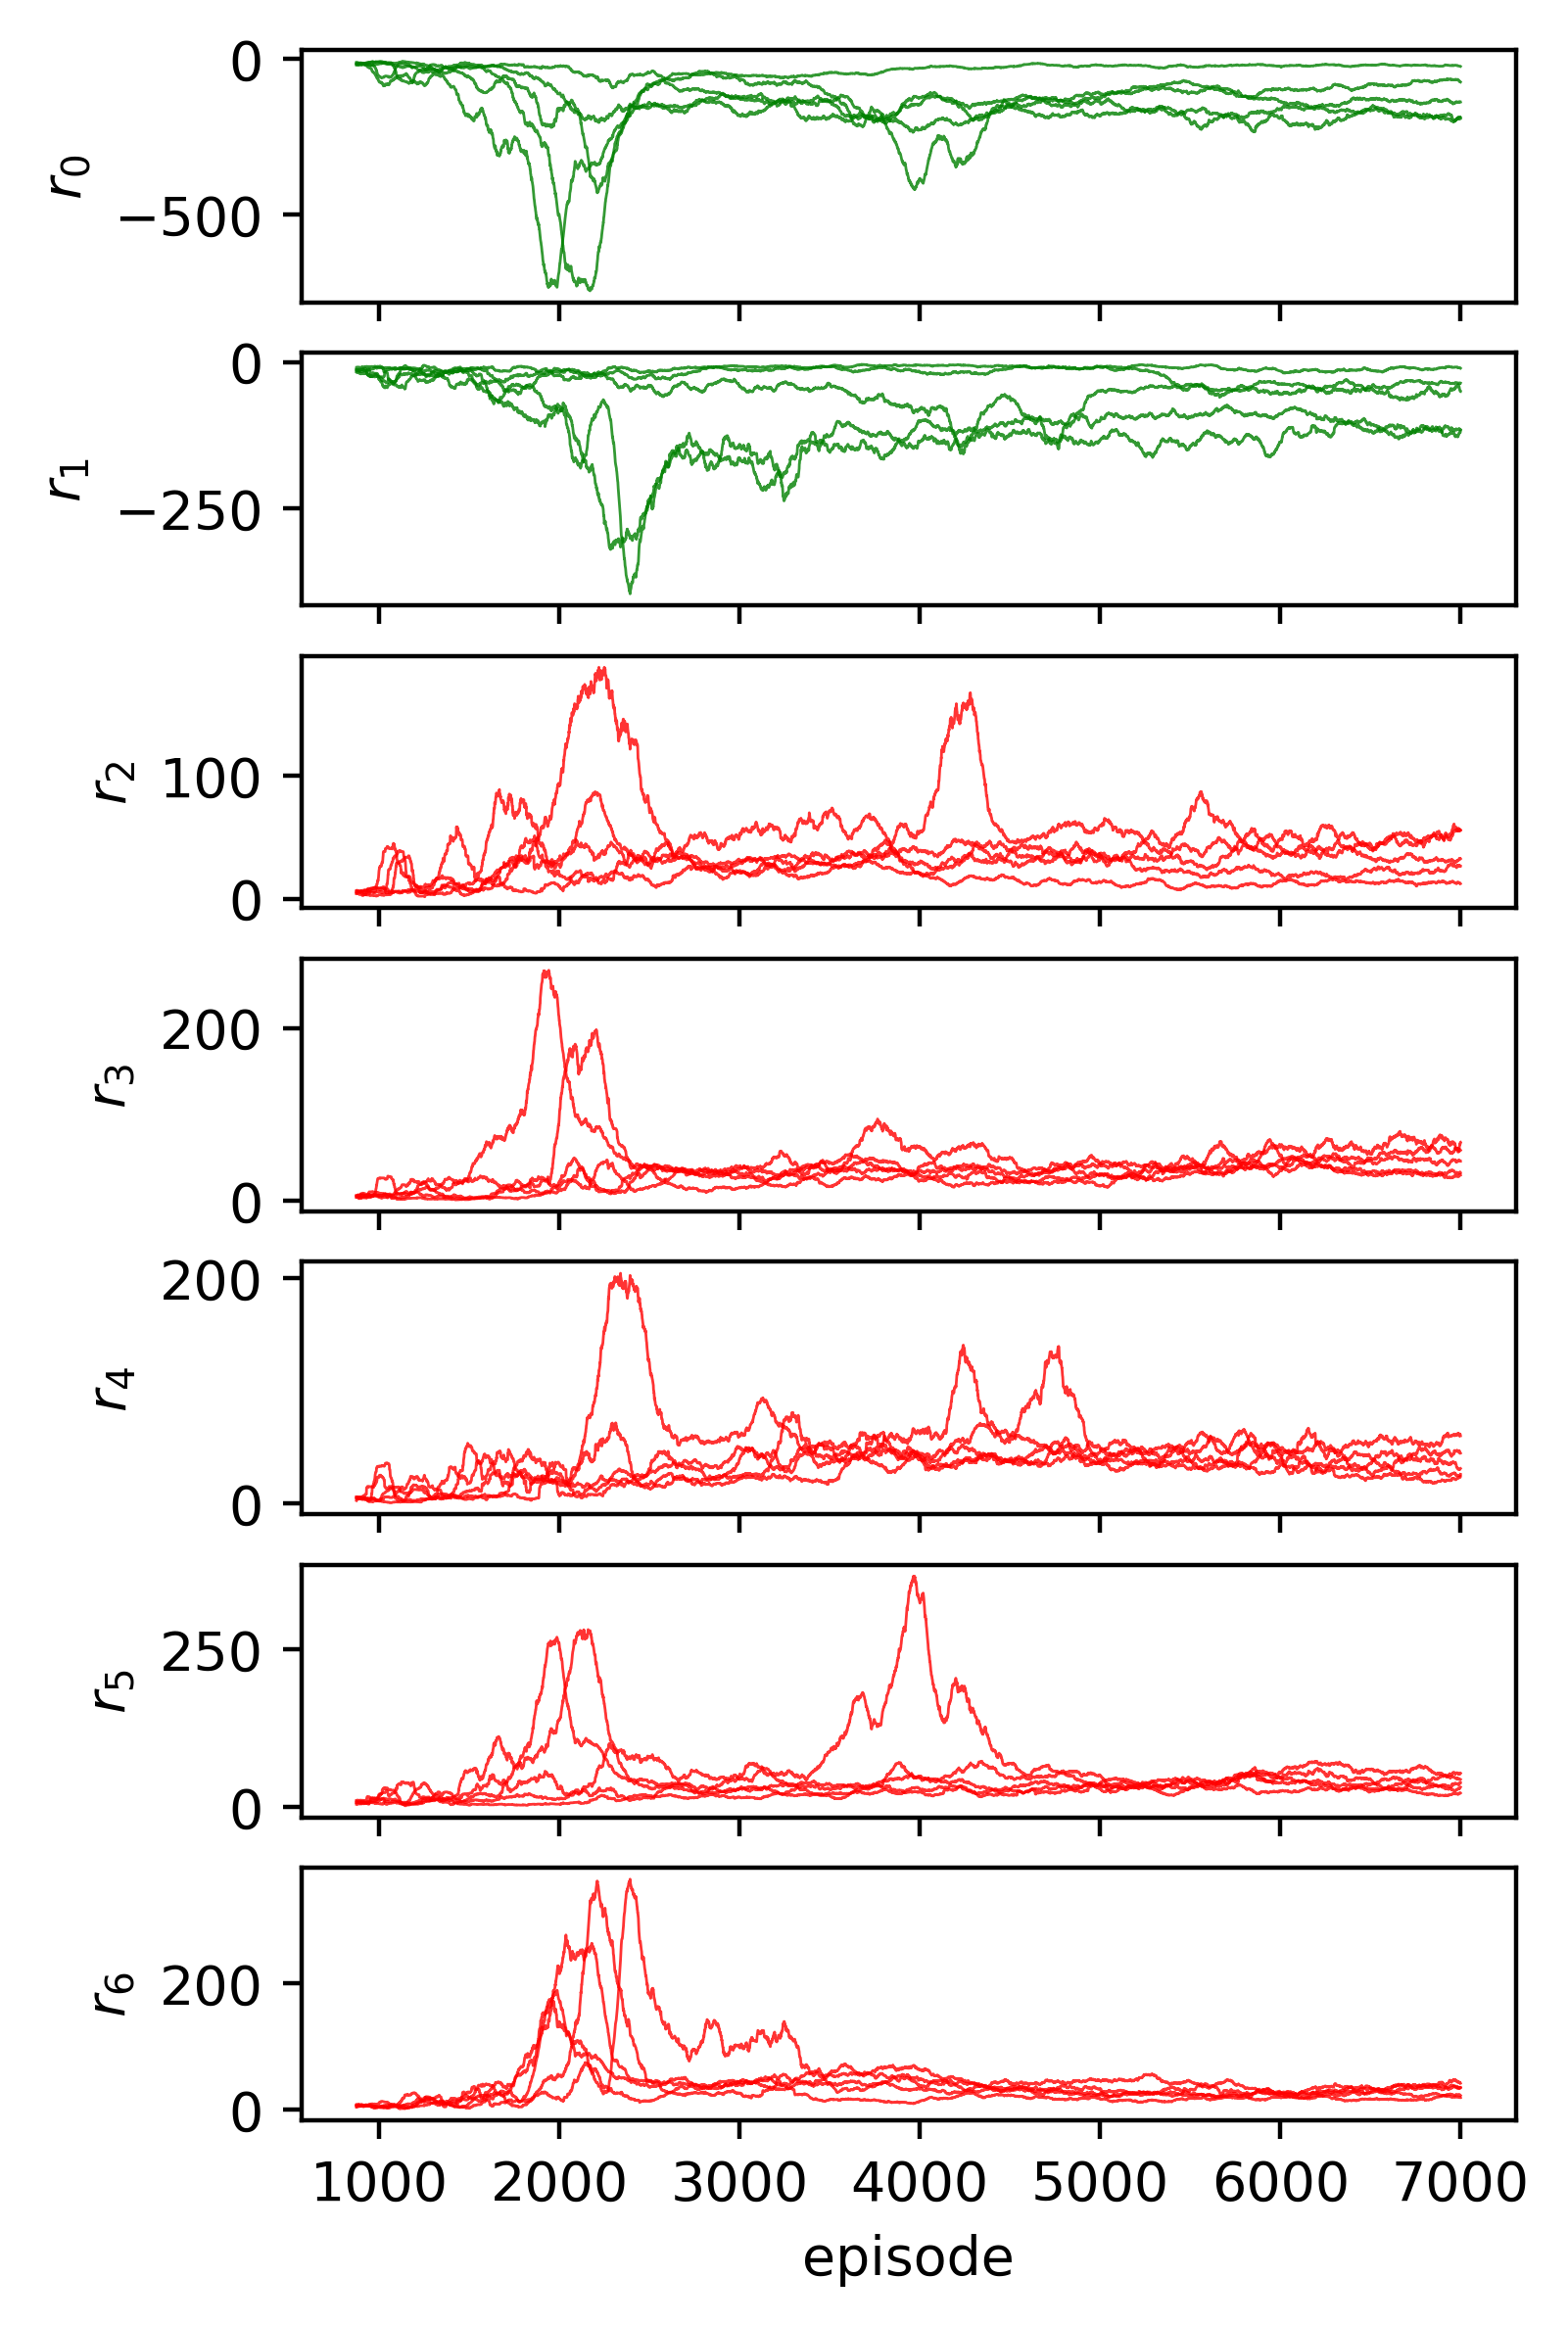
\includegraphics[width=0.5\textwidth]{figures/baseline_reward.png}
  \caption{Reward (moving average over 100 episodes) for survivors (green) and zombies (red) for 10 training runs.}
  \label{fig:baseline_reward}
\end{figure}

There was some variability between training runs in the baseline scenario.
Figure \ref{fig:baseline_reward} shows agent reward graphs over multiple runs.
The reward trace for $r_5$ shows the zombie agent experienced a spike in reward corresponding to a drop in reward for a survivor in $r_0$
that occurred only once in 10 training runs.
Most agents show a similar pattern for at least one run.

On further investigation we discovered the reason for this; a zombie usually fixates on a target, but zombies learn policies at different rates.
Figure \ref{fig:baseline_speed} shows speed and reward over time for a single training run.
We see that one survivor is not pursued as often to start with, but then recieves increasing attention from zombies learning to persure it.
Following this attention the survivor learns to move much faster.
We observed similar patterns in other runs.

In the baseline state-space, every agent is unique, so all agents have to learn their expected reward relating to each other.
From an agent's perspective, when considering reward the most important thing about an agent is whether they are a survivor or a zombie, not necessarily which survivor or zombie.
We'd prefer agents learn general policies that consider other agents exchangeable within a team.

\begin{figure}
  \centering
  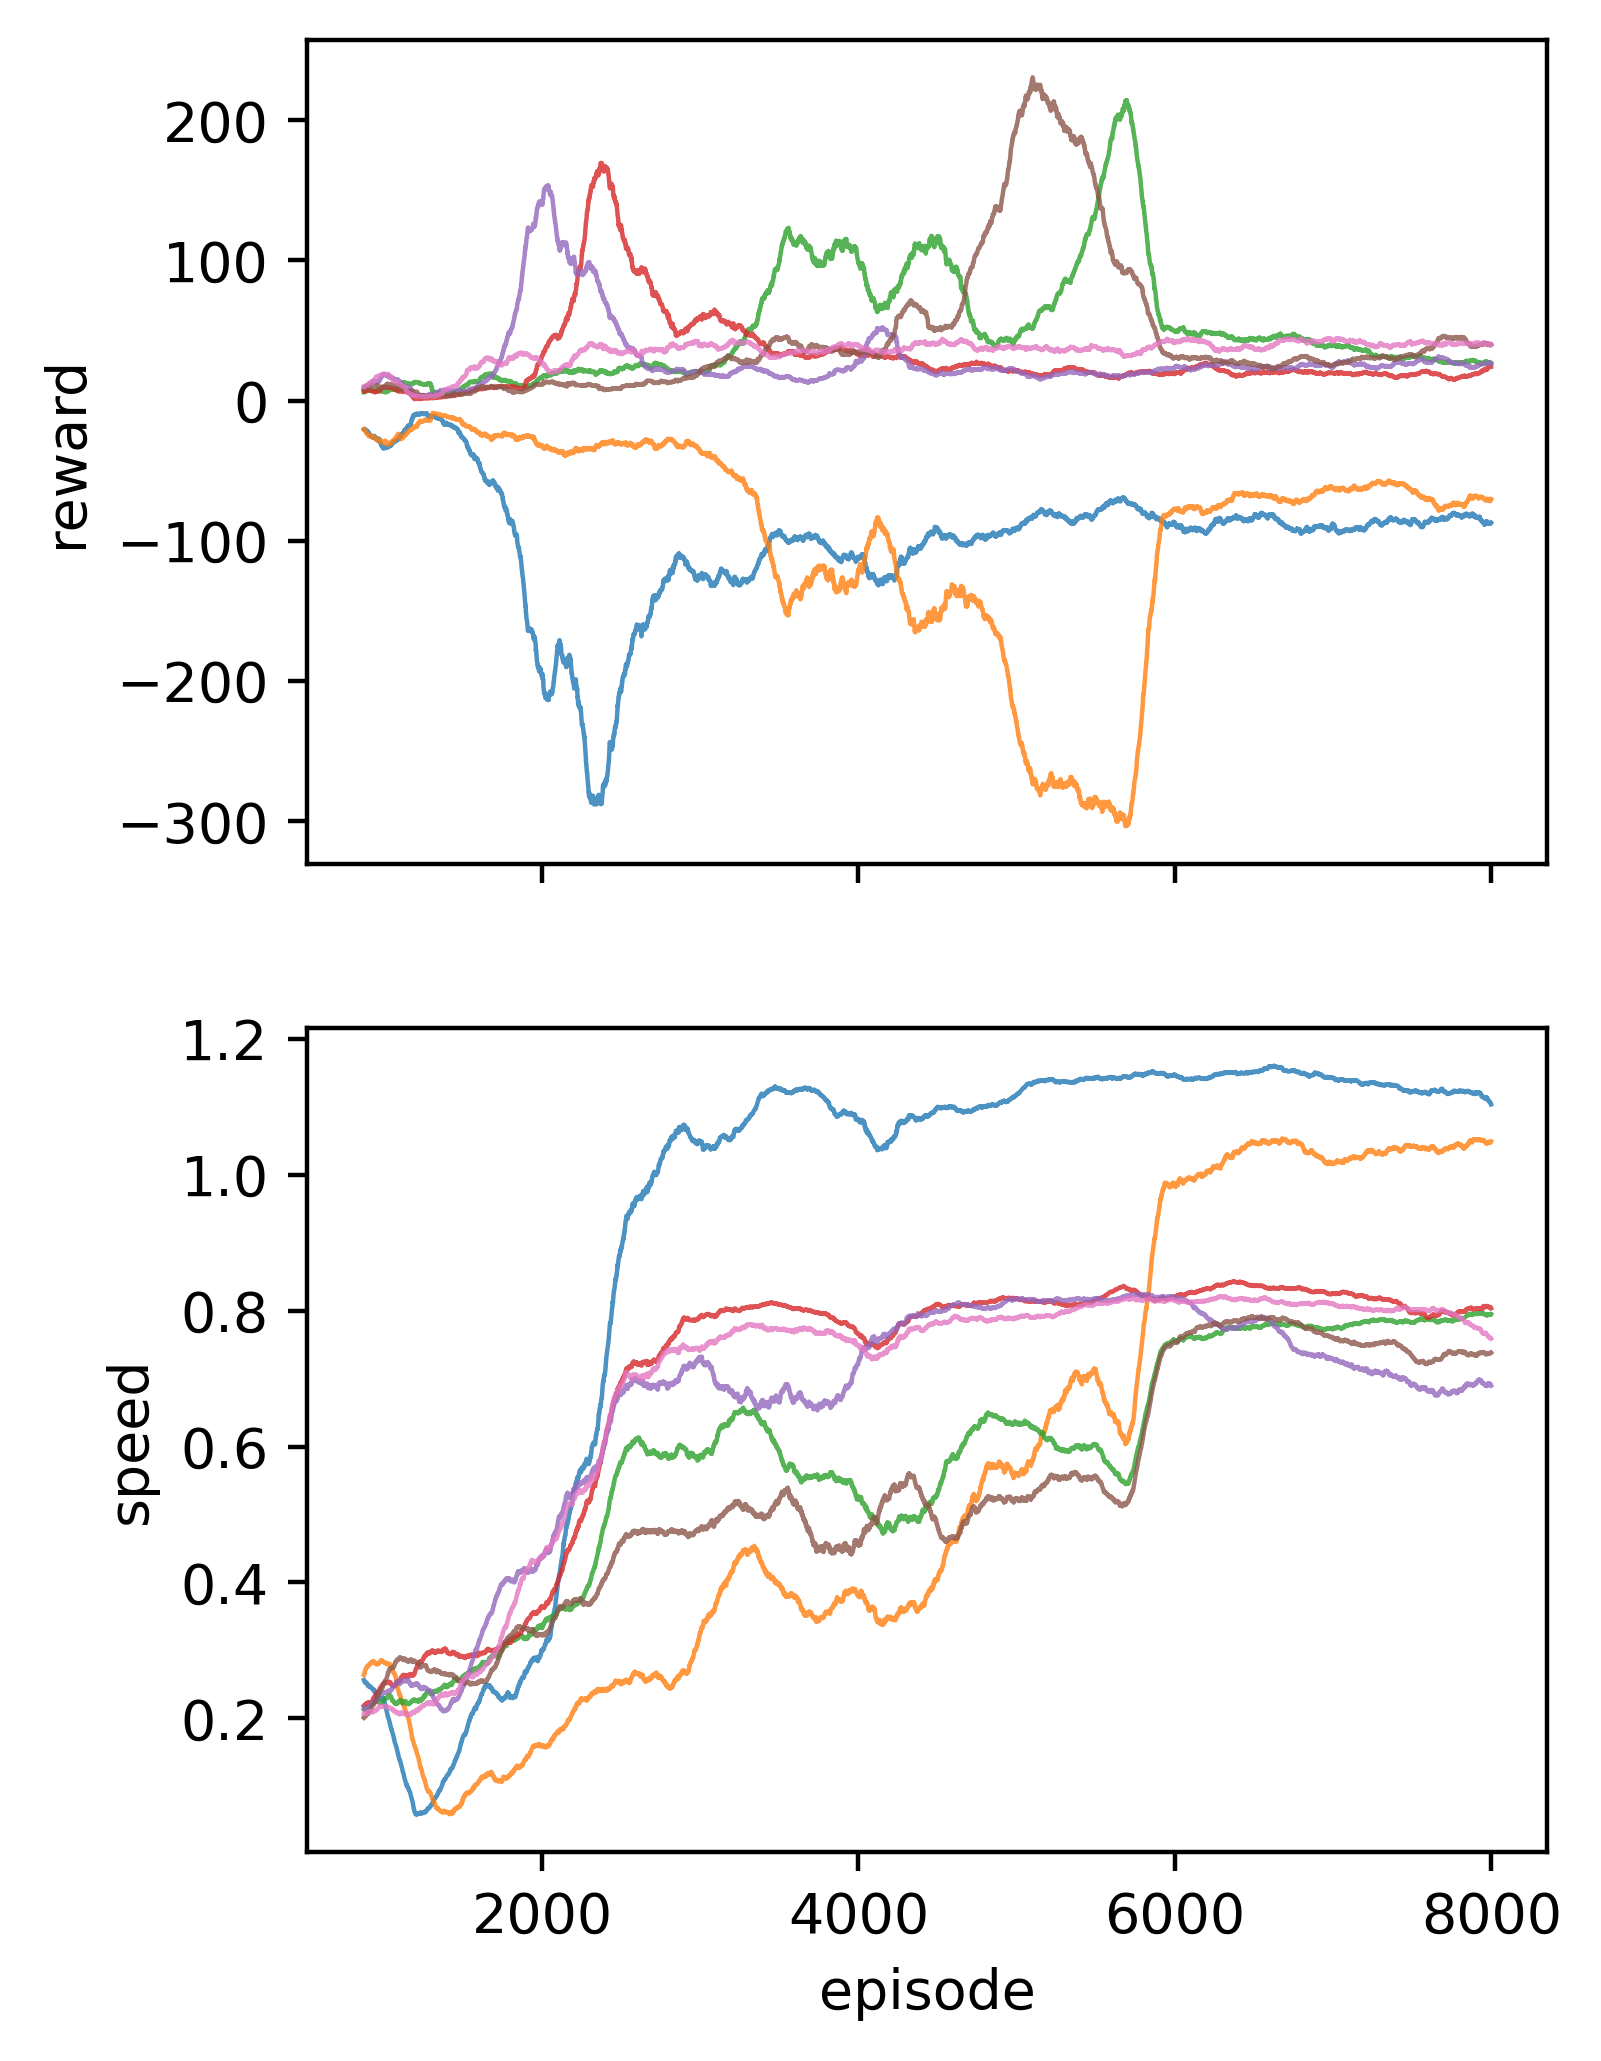
\includegraphics[width=0.5\textwidth]{figures/baseline_speed.png}
  \caption{Moving averages for reward and speed in baseline scenario. Survivors in blue and orange.}
  \label{fig:baseline_speed}
\end{figure}

\subsection{Scenario: Anonymity}
\label{sec:anon}

In the \emph{anonymity} scenario we modify the \emph{baseline} scenario to introduce partial observability.
We re-order agents' state vectors each step so that agents within teams are ordered by distance to the observing agent.
To a survivor, a zombie now appears the same as any other zombie, and does not have identity by virtue of index in the state vector.
This reduces the size of the state-space considerably, and allows agents to learn policies that focus on nearby agents.

We expect both survivors and zombies to learn more general policies with faster convergence than the baseline.
We also expect to see zombies chasing which ever survivor is easiest to chase, rather than fixating on a single survivor.

\subsection{Results: Anonymity}



\subsection{Scenario: Health}
\label{sec:health}

In the \emph{health} scenario we modify the \emph{anonymity} scenario to introduce a health mechanism for survivors.
Survivors start each episode with 100\% health, which for survivors is discounted (by 0.99) every bite.
An agent's health level is added to the private observation space for the agent.
Reward remains the same for bites regardless of health levels,
however maximum speed at each step is limited to the fraction of health remaining.

If a survivor is bitten too often, they become slower than the zombies and risk being overrun, leading to a large amount of bites for the remainder of the episode.
This scenario does not alter the reward function, but increases the variance and magnitude of state-value estimates for both zombies and survivors.
Additionally, this scenario shifts the balance of power heavily toward the zombies.
We expect to see survivor policies emerge that are more risk-averse, and to see zombies elect to chase slower-moving survivors.

\subsection{Results: Health}

\subsection{Scenario: Armed}
\label{sec:arms}

In the \emph{armed} scenario we modify the \emph{health} scenario by arming the survivors with pistols.
Each armed agent has a pistol that fires 2 shots when activated.
On firing, two rays are cast with a small random spread ($\angle p \sim \mathcal{N}(\angle aim, 2^\circ)$) for a range (2m) that covers most of the area.
When a ray first intersects with another agent it is counted as a `hit'.
An agent experiencing a hit has their health level reduced (by 0.2).
Armed agents have a reload time (1 step).
Both zombies and survivors can be rendered immobile through reduced health by being hit too often.

We add a normalized current heading and relative heading of locations of other agents to an armed agent's state space, as well as a normalized time remaining until reloaded.
Reloading is automatic and does not require an action.
The continuous Aiming action (left and right) modifies angular velocity of aim directly up to a maximum speed of 1 revolution per second.
The firing mechanic is implemented as a `tirgger pressure' which determines the probability of a loaded pistol firing in a given timestep.
Firing probability is implemented as the sigmoid function $p(fire) = \frac{1}{1+e^{20(x-0.5)}}$, where $x$ is the pressure on the trigger.

We expect introducing the arms mechanic will move the balance of power back toward the survivors.
We're not sure if the social dilemma presented will cause the survivors to fire on one another more often than the zombies,
but make no adjustment to the reward function to discourage it.

\subsection{Results: Armed}

\section{Discussion}
\label{sec:discussion}

FROM HERE FOLLOWS TEMPLATE STUFF


\paragraph{\LaTeX-specific details:}
To use Times Roman in \LaTeX2e{}, put the following in the preamble:
\begin{quote}
\small
\begin{verbatim}
\usepackage{times}
\usepackage{latexsym}
\end{verbatim}
\end{quote}


\subsection{Ruler}
A printed ruler (line numbers in the left and right margins of the article) should be presented in the version submitted for review, so that reviewers may comment on particular lines in the paper without circumlocution.
The presence or absence of the ruler should not change the appearance of any other content on the page.
The camera ready copy should not contain a ruler.

\paragraph{Reviewers:}
note that the ruler measurements may not align well with lines in the paper -- this turns out to be very difficult to do well when the paper contains many figures and equations, and, when done, looks ugly.
In most cases one would expect that the approximate location will be adequate, although you can also use fractional references (\emph{e.g.}, this line ends at mark $295.5$).

\paragraph{\LaTeX-specific details:}
The style files will generate the ruler when {\small\verb|\aclfinalcopy|} is commented out, and remove it otherwise.

\subsection{Title and Authors}
\label{ssec:title-authors}

Center the title, author's name(s) and affiliation(s) across both columns.
Do not use footnotes for affiliations.
Place the title centered at the top of the first page, in a 15-point bold font.
Long titles should be typed on two lines without a blank line intervening.
Put the title 2.5 cm from the top of the page, followed by a blank line, then the author's names(s), and the affiliation on the following line.
Do not use only initials for given names (middle initials are allowed).
Do not format surnames in all capitals (\emph{e.g.}, use ``Mitchell'' not ``MITCHELL'').
Do not format title and section headings in all capitals except for proper names (such as ``BLEU'') that are
conventionally in all capitals.
The affiliation should contain the author's complete address, and if possible, an electronic mail address.

The title, author names and addresses should be completely identical to those entered to the electronical paper submission website in order to maintain the consistency of author information among all publications of the conference.
If they are different, the publication chairs may resolve the difference without consulting with you; so it is in your own interest to double-check that the information is consistent.

Start the body of the first page 7.5 cm from the top of the page.
\textbf{Even in the anonymous version of the paper, you should maintain space for names and addresses so that they will fit in the final (accepted) version.}


\subsection{Abstract}
Use two-column format when you begin the abstract.
Type the abstract at the beginning of the first column.
The width of the abstract text should be smaller than the
width of the columns for the text in the body of the paper by 0.6 cm on each side.
Center the word \textbf{Abstract} in a 12 point bold font above the body of the abstract.
The abstract should be a concise summary of the general thesis and conclusions of the paper.
It should be no longer than 200 words.
The abstract text should be in 10 point font.

\subsection{Text}
Begin typing the main body of the text immediately after the abstract, observing the two-column format as shown in the present document.

Indent 0.4 cm when starting a new paragraph.

\subsection{Sections}

Format section and subsection headings in the style shown on the present document.
Use numbered sections (Arabic numerals) to facilitate cross references.
Number subsections with the section number and the subsection number separated by a dot, in Arabic numerals.

\subsection{Footnotes}
Put footnotes at the bottom of the page and use 9 point font.
They may be numbered or referred to by asterisks or other symbols.\footnote{This is how a footnote should appear.}
Footnotes should be separated from the text by a line.\footnote{Note the line separating the footnotes from the text.}

\subsection{Graphics}

Place figures, tables, and photographs in the paper near where they are first discussed, rather than at the end, if possible.
Wide illustrations may run across both columns.
Color is allowed, but adhere to Section~\ref{ssec:accessibility}'s guidelines on accessibility.

\paragraph{Captions:}
Provide a caption for every illustration; number each one sequentially in the form:
``Figure 1. Caption of the Figure.''
``Table 1. Caption of the Table.''
Type the captions of the figures and tables below the body, using 10 point text.
Captions should be placed below illustrations.
Captions that are one line are centered (see Table~\ref{font-table}).
Captions longer than one line are left-aligned (see Table~\ref{tab:accents}).

\begin{table}
\centering
\begin{tabular}{lc}
\hline
\textbf{Command} & \textbf{Output}\\
\hline
\verb|{\"a}| & {\"a} \\
\verb|{\^e}| & {\^e} \\
\verb|{\`i}| & {\`i} \\ 
\verb|{\.I}| & {\.I} \\ 
\verb|{\o}| & {\o} \\
\verb|{\'u}| & {\'u}  \\ 
\verb|{\aa}| & {\aa}  \\\hline
\end{tabular}
\begin{tabular}{lc}
\hline
\textbf{Command} & \textbf{Output}\\
\hline
\verb|{\c c}| & {\c c} \\ 
\verb|{\u g}| & {\u g} \\ 
\verb|{\l}| & {\l} \\ 
\verb|{\~n}| & {\~n} \\ 
\verb|{\H o}| & {\H o} \\ 
\verb|{\v r}| & {\v r} \\ 
\verb|{\ss}| & {\ss} \\
\hline
\end{tabular}
\caption{Example commands for accented characters, to be used in, \emph{e.g.}, \BibTeX\ names.}\label{tab:accents}
\end{table}

\paragraph{\LaTeX-specific details:}
The style files are compatible with the caption and subcaption packages; do not add optional arguments.
\textbf{Do not override the default caption sizes.}


\subsection{Hyperlinks}
Within-document and external hyperlinks are indicated with Dark Blue text, Color Hex \#000099.

\subsection{Citations}
Citations within the text appear in parentheses as~\citep{Gusfield:97} or, if the author's name appears in the text itself, as \citet{Gusfield:97}.
Append lowercase letters to the year in cases of ambiguities.  
Treat double authors as in~\citep{Aho:72}, but write as in~\citep{Chandra:81} when more than two authors are involved. Collapse multiple citations as in~\citep{Gusfield:97,Aho:72}. 

Refrain from using full citations as sentence constituents.
Instead of
\begin{quote}
  ``\citep{Gusfield:97} showed that ...''
\end{quote}
write
\begin{quote}
``\citet{Gusfield:97} showed that ...''
\end{quote}

\begin{table*}
\centering
\begin{tabular}{lll}
\hline
\textbf{Output} & \textbf{natbib command} & \textbf{Old ACL-style command}\\
\hline
\citep{Gusfield:97} & \small\verb|\citep| & \small\verb|\cite| \\
\citealp{Gusfield:97} & \small\verb|\citealp| & no equivalent \\
\citet{Gusfield:97} & \small\verb|\citet| & \small\verb|\newcite| \\
\citeyearpar{Gusfield:97} & \small\verb|\citeyearpar| & \small\verb|\shortcite| \\
\hline
\end{tabular}
\caption{\label{citation-guide}
Citation commands supported by the style file.
The style is based on the natbib package and supports all natbib citation commands.
It also supports commands defined in previous ACL style files for compatibility.
}
\end{table*}

\paragraph{\LaTeX-specific details:}
Table~\ref{citation-guide} shows the syntax supported by the style files.
We encourage you to use the natbib styles.
You can use the command {\small\verb|\citet|} (cite in text) to get ``author (year)'' citations as in \citet{Gusfield:97}.
You can use the command {\small\verb|\citep|} (cite in parentheses) to get ``(author, year)'' citations as in \citep{Gusfield:97}.
You can use the command {\small\verb|\citealp|} (alternative cite without  parentheses) to get ``author year'' citations (which is useful for  using citations within parentheses, as in \citealp{Gusfield:97}).


\subsection{References}
Gather the full set of references together under the heading \textbf{References}; place the section before any Appendices. 
Arrange the references alphabetically by first author, rather than by order of occurrence in the text.

Provide as complete a citation as possible, using a consistent format, such as the one for \emph{Computational Linguistics\/} or the one in the  \emph{Publication Manual of the American 
Psychological Association\/}~\citep{APA:83}.
Use full names for authors, not just initials.

Submissions should accurately reference prior and related work, including code and data.
If a piece of prior work appeared in multiple venues, the version that appeared in a refereed, archival venue should be referenced.
If multiple versions of a piece of prior work exist, the one used by the authors should be referenced.
Authors should not rely on automated citation indices to provide accurate references for prior and related work.

The following text cites various types of articles so that the references section of the present document will include them.
\begin{itemize}
\item Example article in journal: \citep{Ando2005}.
\item Example article in proceedings, with location: \citep{borschinger-johnson-2011-particle}.
\item Example article in proceedings, without location: \citep{andrew2007scalable}.
\item Example arxiv paper: \citep{rasooli-tetrault-2015}. 
\end{itemize}


\paragraph{\LaTeX-specific details:}
The \LaTeX{} and Bib\TeX{} style files provided roughly follow the American Psychological Association format.
If your own bib file is named \texttt{\small acl2020.bib}, then placing the following before any appendices in your \LaTeX{}  file will generate the references section for you:
\begin{quote}\small
\verb|\bibliographystyle{acl_natbib}|\\
\verb|\bibliography{acl2020}|
\end{quote}

You can obtain the complete ACL Anthology as a Bib\TeX\ file from \url{https://aclweb.org/anthology/anthology.bib.gz}.
To include both the anthology and your own bib file, use the following instead of the above.
\begin{quote}\small
\verb|\bibliographystyle{acl_natbib}|\\
\verb|\bibliography{anthology,acl2020}|
\end{quote}


\subsection{Digital Object Identifiers}
As part of our work to make ACL materials more widely used and cited outside of our discipline, ACL has registered as a CrossRef member, as a registrant of Digital Object Identifiers (DOIs), the standard for registering permanent URNs for referencing scholarly materials.

All camera-ready references are required to contain the appropriate DOIs (or as a second resort, the hyperlinked ACL Anthology Identifier) to all cited works.
Appropriate records should be found for most materials in the current ACL Anthology at \url{http://aclanthology.info/}.
As examples, we cite \citep{goodman-etal-2016-noise} to show you how papers with a DOI will appear in the bibliography.
We cite \citep{harper-2014-learning} to show how papers without a DOI but with an ACL Anthology Identifier will appear in the bibliography.

\paragraph{\LaTeX-specific details:}
Please ensure that you use Bib\TeX\ records that contain DOI or URLs for any of the ACL materials that you reference.
If the Bib\TeX{} file contains DOI fields, the paper title in the references section will appear as a hyperlink to the DOI, using the hyperref \LaTeX{} package.


\subsection{Appendices}
Appendices, if any, directly follow the text and the
references (but only in the camera-ready; see Appendix~\ref{sec:appendix}).
Letter them in sequence and provide an informative title:
\textbf{Appendix A. Title of Appendix}.

\section{Accessibility}
\label{ssec:accessibility}

In an effort to accommodate people who are color-blind (as well as those printing to paper), grayscale readability is strongly encouraged.
Color is not forbidden, but authors should ensure that tables and figures do not rely solely on color to convey critical distinctions.
A simple criterion:
All curves and points in your figures should be clearly distinguishable without color.

\section{Translation of non-English Terms}

It is also advised to supplement non-English characters and terms with appropriate transliterations and/or translations since not all readers understand all such characters and terms.
Inline transliteration or translation can be represented in the order of:
\begin{center}
\begin{tabular}{c}
original-form \\
transliteration \\
``translation''
\end{tabular}
\end{center}

\section{\LaTeX{} Compilation Issues}
You may encounter the following error during compilation: 
\begin{quote}
{\small\verb|\pdfendlink|} ended up in different nesting level than {\small\verb|\pdfstartlink|}.
\end{quote}
This happens when \texttt{\small pdflatex} is used and a citation splits across a page boundary.
To fix this, the style file contains a patch consisting of two lines:
(1) {\small\verb|\RequirePackage{etoolbox}|} (line 455 in \texttt{\small acl2020.sty}), and
(2) A long line below (line 456 in \texttt{\small acl2020.sty}).

If you still encounter compilation issues even with the patch enabled, disable the patch by commenting the two lines, and then disable the \texttt{\small hyperref} package by loading the style file with the \texttt{\small nohyperref} option:

\noindent
{\small\verb|\usepackage[nohyperref]{acl2020}|}

\noindent
Then recompile, find the problematic citation, and rewrite the sentence containing the citation. (See, {\em e.g.}, \url{http://tug.org/errors.html})

\section*{Acknowledgments}

The acknowledgments should go immediately before the references. Do not number the acknowledgments section.
Do not include this section when submitting your paper for review.

\bibliography{anthology,acl2020}
\bibliographystyle{acl_natbib}

\appendix

\section{Appendices}
\label{sec:appendix}
Appendices are material that can be read, and include lemmas, formulas, proofs, and tables that are not critical to the reading and understanding of the paper. 
Appendices should be \textbf{uploaded as supplementary material} when submitting the paper for review.
Upon acceptance, the appendices come after the references, as shown here.

\paragraph{\LaTeX-specific details:}
Use {\small\verb|\appendix|} before any appendix section to switch the section numbering over to letters.


\section{Supplemental Material}
\label{sec:supplemental}
Submissions may include non-readable supplementary material used in the work and described in the paper.
Any accompanying software and/or data should include licenses and documentation of research review as appropriate.
Supplementary material may report preprocessing decisions, model parameters, and other details necessary for the replication of the experiments reported in the paper.
Seemingly small preprocessing decisions can sometimes make a large difference in performance, so it is crucial to record such decisions to precisely characterize state-of-the-art methods. 

Nonetheless, supplementary material should be supplementary (rather than central) to the paper.
\textbf{Submissions that misuse the supplementary material may be rejected without review.}
Supplementary material may include explanations or details of proofs or derivations that do not fit into the paper, lists of
features or feature templates, sample inputs and outputs for a system, pseudo-code or source code, and data.
(Source code and data should be separate uploads, rather than part of the paper).

The paper should not rely on the supplementary material: while the paper may refer to and cite the supplementary material and the supplementary material will be available to the reviewers, they will not be asked to review the supplementary material.

\end{document}
